\documentclass[sigconf]{acmart}

\usepackage{tikz}
\usetikzlibrary{arrows.meta,positioning}

\AtBeginDocument{%
  \providecommand\BibTeX{{%
    Bib\TeX}}}

\setcopyright{none}
\copyrightyear{2026}
\acmYear{2026}
\acmConference[ASE 2026]{Proceedings of the 41st IEEE/ACM International Conference on Automated Software Engineering}{October 12--16, 2026}{Munich, Germany}
\acmBooktitle{Proceedings of the 41st IEEE/ACM International Conference on Automated Software Engineering (ASE 2026), October 12--16, 2026, Munich, Germany}
% \acmDOI is intentionally omitted during submission drafting. The Zenodo
% artifact DOI appears in the abstract and Data Availability Statement.
\acmISBN{TBD}

\title{ErrPilot: Auditable Failure Provenance and Handoff for AI-Assisted Debugging}

\author{Yangchenxi Wu}
\affiliation{%
  \institution{Hungarian University of Sports Science}
  \city{Budapest}
  \country{Hungary}}
\email{wuyang778@gmail.com}

\begin{document}

\begin{abstract}
ErrPilot is a CLI-first tool for turning explicitly wrapped failing commands
into auditable failure provenance for AI-assisted debugging workflows. Rather
than acting as a repair agent, ErrPilot standardizes the intake layer before a
human or downstream coding tool investigates a failure: what command failed,
what raw evidence was captured, what source context was selected, what local
routing decision was made, and what verification contract accompanies a handoff.
It captures command metadata, preserves raw stdout/stderr logs while exposing
compact structured excerpts, parses Python traceback and pytest failure signals,
extracts bounded source contexts, runs deterministic local triage, and generates
reviewable handoff prompts. The artifact is local-first and reproducible: it
requires no external service calls, does not silently monitor terminal activity,
and does not execute downstream repair tools. We evaluate ErrPilot with 7
open-source, repository-local executable failure cases covering pytest assertions,
fixture/setup failures, imports, multi-test failures, missing configuration,
type errors, and standalone tracebacks. A deterministic handoff-quality probe on
all 7 cases shows that raw failure prompts contain only 2/7 required handoff
fields on average, while ErrPilot handoff artifacts contain 7/7. We also report one
optional cross-project vignette on the public SkiLoadLab Python CLI.
Artifact: \url{https://doi.org/10.5281/zenodo.20053341}. Video:
\url{https://youtu.be/-cGRD9A6AXo}.
\end{abstract}

\begin{CCSXML}
<ccs2012>
   <concept>
       <concept_id>10011007.10011074.10011099</concept_id>
       <concept_desc>Software and its engineering~Software testing and debugging</concept_desc>
       <concept_significance>500</concept_significance>
       </concept>
   <concept>
       <concept_id>10011007.10011006.10011008</concept_id>
       <concept_desc>Software and its engineering~General programming languages</concept_desc>
       <concept_significance>300</concept_significance>
       </concept>
</ccs2012>
\end{CCSXML}

\ccsdesc[500]{Software and its engineering~Software testing and debugging}
\ccsdesc[300]{Software and its engineering~General programming languages}
\keywords{failure intake, debugging, software artifacts, triage, AI-assisted software engineering}

\maketitle

\section{Introduction}

Modern AI-assisted debugging workflows often begin from an unstructured failure:
a test run, traceback, build log, or CI excerpt is pasted into a human review or
coding-agent session~\cite{swe-agent}. This intake step is easy to
under-specify. The prompt may omit command metadata, lose raw evidence, include
excessive logs, or fail to record the local source context and verification
contract needed to audit a suggested repair.

ErrPilot addresses this intake problem. It is a CLI-first failure provenance and
handoff tool that turns explicitly wrapped failing commands into structured,
auditable records. ErrPilot is not a repair agent. It does not modify source
code, apply patches, execute downstream coding tools, or silently monitor
terminal activity. Instead, it captures the failure, extracts structured local
evidence, runs deterministic local triage, and emits reviewable handoff prompts
for humans or downstream tools.

ErrPilot complements existing failure surfaces rather than replacing them.
Terminal output and CI logs preserve evidence, but they do not provide a stable,
structured intake object. Issue templates encourage structure, but rely on
manual completion. Coding agents and automated repair systems can consume
failure evidence~\cite{swe-agent,legoues-genprog}, but the evidence is often
pasted ad hoc. ErrPilot addresses the intermediate layer: it constructs a
repeatable provenance object before repair or investigation begins, so later
actions can be traced back to captured evidence and an explicit handoff record.

This demonstration paper makes four contributions:
\begin{itemize}
  \item a structured failure provenance schema separating raw evidence, parsed
  diagnostics, bounded source contexts, triage records, and handoff artifacts;
  \item a CLI workflow for explicit run capture, bundle construction,
  deterministic local triage, and reviewable handoff prompt generation;
  \item a bounded source-context extraction policy for Python traceback and
  pytest failures without copying complete source files into the bundle; and
  \item a reproducible artifact-readiness evaluation with 7 executable local
  cases, a deterministic handoff-quality probe quantifying provenance
  completeness over raw prompts, one optional cross-project vignette,
  documented design probes, CI checks, and optional Docker validation.
\end{itemize}

\section{Tool Overview}

ErrPilot is used as an explicit wrapper around a command selected by the user:
\begin{verbatim}
errpilot run -- pytest \
  examples/python_assertion_failure
errpilot bundle latest
errpilot triage latest --local
errpilot route latest --target codex
\end{verbatim}
The first command records stdout, stderr, a combined log, command text, exit
status, and timing metadata under a run directory. Subsequent commands construct
a human-readable and machine-readable bundle, expose repository state in the
bundle, attach local triage, and write a target-specific prompt artifact.
ErrPilot executes only the user-supplied command explicitly passed to
\texttt{errpilot run --}; it does not sandbox that command.

\begin{figure}[t]
  \centering
  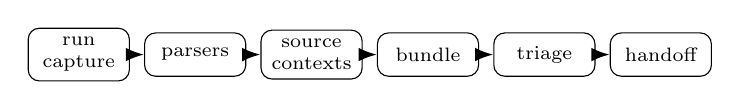
\begin{tikzpicture}[
    node distance=0.18cm,
    pipelinebox/.style={draw, rounded corners, align=center, font=\scriptsize,
      minimum height=0.55cm, text width=1.05cm},
    arrow/.style={-Latex, thick}
  ]
    \node[pipelinebox] (capture) {run\\capture};
    \node[pipelinebox, right=of capture] (parsers) {parsers};
    \node[pipelinebox, right=of parsers] (contexts) {source\\contexts};
    \node[pipelinebox, right=of contexts] (bundle) {bundle};
    \node[pipelinebox, right=of bundle] (triage) {triage};
    \node[pipelinebox, right=of triage] (handoff) {handoff};
    \draw[arrow] (capture) -- (parsers);
    \draw[arrow] (parsers) -- (contexts);
    \draw[arrow] (contexts) -- (bundle);
    \draw[arrow] (bundle) -- (triage);
    \draw[arrow] (triage) -- (handoff);
  \end{tikzpicture}
  \caption{ErrPilot failure intake pipeline from explicit command capture to
  structured bundle generation, deterministic triage, and reviewable handoff
  prompt creation.}
  \Description{Pipeline from failed command to run capture, parsing, source
  context extraction, error bundle generation, local triage, and handoff prompt.}
  \label{fig:pipeline}
\end{figure}

\section{Failure Bundle Schema and Workflow}

ErrPilot stores raw evidence as files and exposes structured diagnosis fields in
\texttt{error\_bundle.json}. The stable top-level fields include run metadata,
the wrapped command, log paths and compact excerpts, git state, parsed Python
traceback information, pytest failing tests, bounded source contexts, risk
flags, local triage, and handoff artifact records. A companion
\texttt{error\_bundle.md} provides a readable review surface.

\begin{table}[t]
  \caption{Failure bundle schema groups. Raw evidence remains on disk while the
  JSON bundle exposes compact, auditable fields for tools and reviewers.}
  \label{tab:schema}
  \small
  \begin{tabular}{p{0.16\linewidth}p{0.34\linewidth}p{0.36\linewidth}}
    \toprule
    Group & Fields & Purpose \\
    \midrule
    Run & \texttt{command}, \texttt{cwd}, \texttt{exit\_code}, \texttt{run\_id}
      & failed command context \\
    Logs & stdout/stderr paths, compact excerpts
      & raw evidence plus compact review view \\
    Diagnostics & \texttt{python\_traceback}, \texttt{pytest}, \texttt{failing\_tests}
      & parsed failure signals \\
    Context & \texttt{source\_contexts}
      & bounded code windows \\
    State & \texttt{git}
      & branch, commit, dirty status \\
    Handoff & \texttt{triage}, \texttt{handoff\_artifacts}
      & routing and prompt outputs \\
    \bottomrule
  \end{tabular}
\end{table}

The bundle is intentionally organized for auditability. Raw logs remain
available as separate files, while prompt artifacts use structured fields and
bounded excerpts. Very small logs may fit entirely inside an excerpt; the design
goal is bounded evidence, not a guarantee that no complete small log can appear.
Sensitive paths such as \texttt{.env}, private keys, token files, and credential
files are excluded from source-context collection by default.

\paragraph{Design policies.}
ErrPilot applies deterministic intake policies rather than learned ranking. For
pytest output, it records failing node identifiers, file paths, test names, and
error classes when those signals are present. For Python tracebacks, it selects
repository-local frames and ignores external library frames for source-context
collection. Source windows are bounded around the failing line and carry a role
label such as \texttt{failing\_test} or \texttt{traceback}; complete files are
not copied into handoff prompts. Local triage applies ordered rules over parsed
signals such as missing imports, missing files, fixture/setup failures,
multi-test failures, and local assertion or type errors. Handoff generation then
renders the structured bundle into a target-specific artifact that includes a
verification command and constraints, but does not invoke the target.

Local triage is deterministic and rule-based. It records severity, confidence,
recommended route, reason, and a human-approval requirement. Route generation
then writes prompt artifacts for targets such as Codex, Aider, Gemini CLI, or
manual review. These prompt files are artifacts for inspection and handoff;
ErrPilot does not execute downstream repair tools.

\begin{table}[t]
  \caption{Positioning against common failure-handling workflows.}
  \label{tab:positioning}
  \small
  \begin{tabular}{p{0.25\linewidth}p{0.29\linewidth}p{0.33\linewidth}}
    \toprule
    Surface & Strength & Gap addressed by ErrPilot \\
    \midrule
    Terminal / CI logs & preserve raw output & no reusable structured bundle \\
    Issue templates & encourage structure & manually completed evidence \\
    Agent prompts & immediate handoff & weak audit trail \\
    Repair agents & can investigate or patch & execute after intake; not a record format \\
    ErrPilot & structured local intake & stops before repair, stores auditable artifacts \\
    \bottomrule
  \end{tabular}
\end{table}

\section{Evaluation and Artifact Readiness}

We provide a reproducible artifact-readiness evaluation augmented with a
deterministic handoff-quality probe that quantifies the provenance advantage of
ErrPilot handoff artifacts over raw failure prompts. The evaluation asks whether
each executable failure can be captured, normalized, triaged, routed, and
reproduced without relying on external services or downstream repair tools.

For the handoff-quality probe, we run the same checklist over all 7 executable
failures. The
probe compares a raw-log prompt against the generated Codex handoff artifact
and checks whether the input explicitly contains seven fields needed for a
controlled debugging handoff: expected error, relevant file, verification
command, source context, triage route, human-approval gate, and safety
constraints. This probe does not ask an LLM or human to repair the bug; it
measures whether the handoff artifact carries the evidence and guardrails that a
downstream workflow would otherwise need to reconstruct.

\begin{table}[t]
  \caption{Artifact-readiness criteria exercised by the 7 executable
  open-source, repository-local cases.}
  \label{tab:evaluation}
  \small
  \begin{tabular}{p{0.22\linewidth}p{0.43\linewidth}p{0.17\linewidth}}
    \toprule
    Criterion & Evidence checked & Coverage \\
    \midrule
    Capture & logs, command, metadata, exit code & 7/7 cases \\
    Parsing & pytest failures or Python traceback fields & 7/7 cases \\
    Context & bounded repository-local source windows & 7/7 cases \\
    Triage & severity, route, confidence, approval flag & 7/7 cases \\
    Handoff & prompt artifact plus verification command & 7/7 cases \\
    Reproduction & tests, lint, evaluation, demo path & check script \\
    \bottomrule
  \end{tabular}
\end{table}

\begin{table}[t]
  \caption{Deterministic handoff-quality probe on all 7 executable cases. Scores count explicit
  fields present in the input artifact, not repair success.}
  \label{tab:handoff-probe}
  \small
  \begin{tabular}{p{0.30\linewidth}p{0.19\linewidth}p{0.33\linewidth}}
    \toprule
    Input artifact & Mean score & Missing from raw log \\
    \midrule
    Raw failure prompt & 2.0/7 & verification contract; bounded source context;
      triage and safety constraints \\
    ErrPilot handoff & 7.0/7 & no checked provenance fields missing \\
    \bottomrule
  \end{tabular}
\end{table}

This demonstrates that ErrPilot systematically closes a provenance gap that raw
failure logs leave for controlled downstream debugging handoff.

The 7 executable cases are open-source examples maintained inside the artifact
repository and are the primary reproducible evidence. They cover pytest
assertions, fixture/setup failures, import failures, multi-test failures, missing
configuration, type errors, and standalone Python tracebacks. All 7 produce raw
run artifacts, structured bundles, bounded source contexts, local triage records,
and reviewable handoff artifacts.

We additionally ran an optional cross-project vignette against the public
SkiLoadLab Python package~\cite{skiloadlab}. The command invoked its documented
\texttt{skiloadlab.cli.combine} entry point with a deterministic missing CSV
input under \texttt{/tmp}. ErrPilot captured the file-missing traceback,
selected repository-local contexts in the CLI wrapper and core model, produced
local triage with severity 4 and a human-approval gate, and generated a Codex
handoff artifact. This is a vignette, not a repair benchmark: it demonstrates
that the intake workflow transfers to a separate open-source Python CLI without
requiring external services.

The remaining documented-only external entries are design probes from
SkiLoadLab and slsa-verifier contexts. They are included to motivate CI, shell,
and supply-chain failure categories for future work. They are not executed by
default, avoid external repository paths, archived CI state, network calls, and
mutation, and are excluded from all default executable artifact-readiness
claims.

Artifact readiness is checked in three paths: a clean-clone virtual environment
path that runs tests, lint, evaluation, and a minimal CLI demo; a one-command
artifact-check script covering the same steps; and an optional Docker path that
builds a local image and runs the artifact check without publishing images or
requiring Docker Hub credentials. The GitHub Actions workflow separates the
Python validation job from the Docker validation job~\cite{github-actions}.
The Docker path follows common containerized artifact practice~\cite{docker},
but it is optional; the clean clone plus virtual environment path remains the
primary reproduction route.

The artifact is archived on Zenodo and is intended to satisfy the spirit of ACM
artifact availability guidance: reviewers can retrieve a versioned object with a
DOI and exercise the included scripts without external services~\cite{acm-badging}.
The version-specific snapshot is separate from the live GitHub repository so
that paper claims can be tied to a stable release.

At the time of writing, the public repository includes a passing Python CI job,
a passing Docker validation job, a Zenodo archive, and a one-command artifact
check script.

The executable cases are intentionally small and deterministic, which improves
artifact reproducibility but limits ecological validity. They are open-source
cases in the artifact repository rather than closed synthetic fixtures, but they
do not establish downstream repair success or field performance. The SkiLoadLab
vignette is a single cross-project sanity check, not evidence of general field
performance. The documented external probes motivate broader categories only.

\section{Limitations}

ErrPilot does not repair bugs, rank patches, or measure downstream agent
success. It standardizes failure intake and handoff before repair, rather than
competing with repair agents. The evaluation is an artifact-readiness study, not
a broad empirical benchmark or downstream-agent comparison. The external
SkiLoadLab vignette is optional and single-case; slsa-verifier entries are
documented-only design probes and are not reproduced by the default evaluation.
Local triage is deterministic and intentionally simple. ErrPilot executes
user-supplied commands explicitly passed to \texttt{errpilot run --}; it does
not sandbox those commands. Future work should measure downstream agent
diagnosis and repair outcomes with and without ErrPilot bundles.

\section{Data Availability Statement}

ErrPilot, its documentation, executable examples, evaluation case metadata,
generated evaluation results, artifact reproduction scripts, CI workflow, and
optional Docker reproduction path are available in the public repository at
\url{https://github.com/YangchenxiWu/errpilot} and archived on Zenodo at
\url{https://doi.org/10.5281/zenodo.20053341}. The default artifact evaluation
uses only in-repository examples and does not require external repositories,
external APIs, secrets, or downstream repair tools. The SkiLoadLab vignette is
provided as an optional cross-project check, while other external cases remain
documented-only metadata for context and are not executed by default.

\begin{thebibliography}{9}

\bibitem{errpilot-artifact}
Yangchenxi Wu.
\newblock ErrPilot artifact repository.
\newblock Version-specific archival artifact snapshot:
\url{https://doi.org/10.5281/zenodo.20053341}, 2026.

\bibitem{skiloadlab}
Yangchenxi Wu.
\newblock SkiLoadLab: reproducible training load modeling for downhill skiing.
\newblock \url{https://github.com/YangchenxiWu/SkiLoadLab}, 2026.

\bibitem{pytest}
pytest developers.
\newblock pytest documentation.
\newblock \url{https://docs.pytest.org/}.

\bibitem{docker}
Docker Inc.
\newblock Docker documentation.
\newblock \url{https://docs.docker.com/}.

\bibitem{github-actions}
GitHub.
\newblock GitHub Actions documentation.
\newblock \url{https://docs.github.com/actions}.

\bibitem{swe-agent}
John Yang, Carlos E. Jimenez, Alexander Wettig, Kilian Lieret, Shunyu Yao,
Karthik Narasimhan, and Ofir Press.
\newblock SWE-agent: Agent-Computer Interfaces Enable Automated Software
Engineering.
\newblock \emph{Advances in Neural Information Processing Systems}, 37, 2024.
\newblock \url{https://doi.org/10.52202/079017-1601}.

\bibitem{legoues-genprog}
Claire Le Goues, ThanhVu Nguyen, Stephanie Forrest, and Westley Weimer.
\newblock GenProg: A Generic Method for Automatic Software Repair.
\newblock \emph{IEEE Transactions on Software Engineering}, 38(1):54--72, 2012.
\newblock \url{https://doi.org/10.1109/TSE.2011.104}.

\bibitem{acm-badging}
ACM Publications Board.
\newblock Artifact review and badging policy.
\newblock \url{https://www.acm.org/publications/policies/artifact-review-and-badging-current}.

\end{thebibliography}

\end{document}
